% Created by tikzDevice version 0.10.1 on 2016-08-29 18:23:12
% !TEX encoding = UTF-8 Unicode
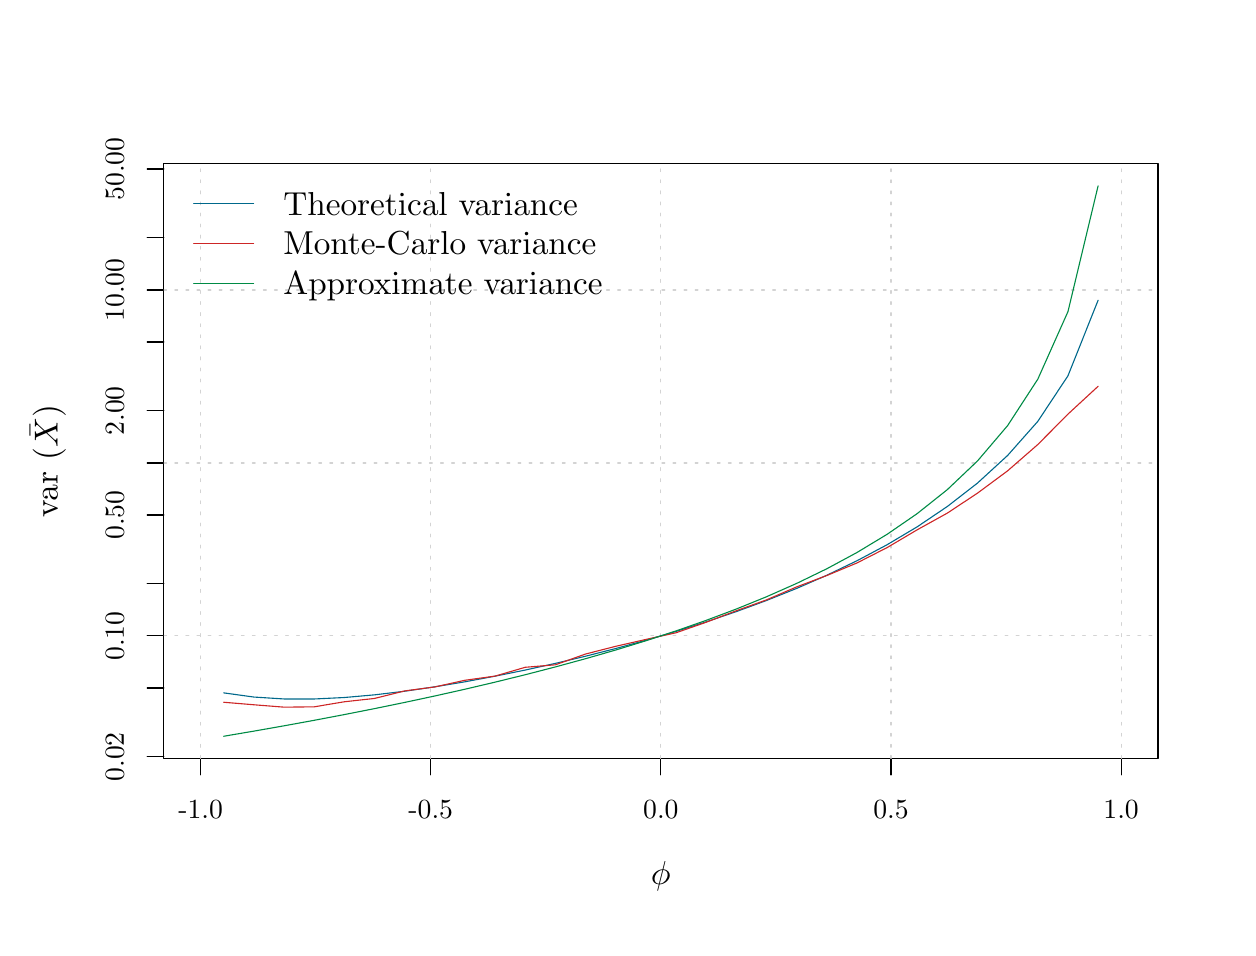
\begin{tikzpicture}[x=1pt,y=1pt]
\definecolor{fillColor}{RGB}{255,255,255}
\path[use as bounding box,fill=fillColor,fill opacity=0.00] (0,0) rectangle (433.62,325.21);
\begin{scope}
\path[clip] (  0.00,  0.00) rectangle (433.62,325.21);
\definecolor{drawColor}{RGB}{0,0,0}

\path[draw=drawColor,line width= 0.4pt,line join=round,line cap=round] ( 62.50, 61.20) -- (395.12, 61.20);

\path[draw=drawColor,line width= 0.4pt,line join=round,line cap=round] ( 62.50, 61.20) -- ( 62.50, 55.20);

\path[draw=drawColor,line width= 0.4pt,line join=round,line cap=round] (145.66, 61.20) -- (145.66, 55.20);

\path[draw=drawColor,line width= 0.4pt,line join=round,line cap=round] (228.81, 61.20) -- (228.81, 55.20);

\path[draw=drawColor,line width= 0.4pt,line join=round,line cap=round] (311.96, 61.20) -- (311.96, 55.20);

\path[draw=drawColor,line width= 0.4pt,line join=round,line cap=round] (395.12, 61.20) -- (395.12, 55.20);

\node[text=drawColor,anchor=base,inner sep=0pt, outer sep=0pt, scale=  1.00] at ( 62.50, 39.60) {-1.0};

\node[text=drawColor,anchor=base,inner sep=0pt, outer sep=0pt, scale=  1.00] at (145.66, 39.60) {-0.5};

\node[text=drawColor,anchor=base,inner sep=0pt, outer sep=0pt, scale=  1.00] at (228.81, 39.60) {0.0};

\node[text=drawColor,anchor=base,inner sep=0pt, outer sep=0pt, scale=  1.00] at (311.96, 39.60) {0.5};

\node[text=drawColor,anchor=base,inner sep=0pt, outer sep=0pt, scale=  1.00] at (395.12, 39.60) {1.0};

\path[draw=drawColor,line width= 0.4pt,line join=round,line cap=round] ( 49.20, 61.72) -- ( 49.20,274.12);

\path[draw=drawColor,line width= 0.4pt,line join=round,line cap=round] ( 49.20, 61.72) -- ( 43.20, 61.72);

\path[draw=drawColor,line width= 0.4pt,line join=round,line cap=round] ( 49.20, 86.60) -- ( 43.20, 86.60);

\path[draw=drawColor,line width= 0.4pt,line join=round,line cap=round] ( 49.20,105.41) -- ( 43.20,105.41);

\path[draw=drawColor,line width= 0.4pt,line join=round,line cap=round] ( 49.20,124.23) -- ( 43.20,124.23);

\path[draw=drawColor,line width= 0.4pt,line join=round,line cap=round] ( 49.20,149.10) -- ( 43.20,149.10);

\path[draw=drawColor,line width= 0.4pt,line join=round,line cap=round] ( 49.20,167.92) -- ( 43.20,167.92);

\path[draw=drawColor,line width= 0.4pt,line join=round,line cap=round] ( 49.20,186.74) -- ( 43.20,186.74);

\path[draw=drawColor,line width= 0.4pt,line join=round,line cap=round] ( 49.20,211.61) -- ( 43.20,211.61);

\path[draw=drawColor,line width= 0.4pt,line join=round,line cap=round] ( 49.20,230.43) -- ( 43.20,230.43);

\path[draw=drawColor,line width= 0.4pt,line join=round,line cap=round] ( 49.20,249.24) -- ( 43.20,249.24);

\path[draw=drawColor,line width= 0.4pt,line join=round,line cap=round] ( 49.20,274.12) -- ( 43.20,274.12);

\node[text=drawColor,rotate= 90.00,anchor=base,inner sep=0pt, outer sep=0pt, scale=  1.00] at ( 34.80, 61.72) {0.02};

\node[text=drawColor,rotate= 90.00,anchor=base,inner sep=0pt, outer sep=0pt, scale=  1.00] at ( 34.80,105.41) {0.10};

\node[text=drawColor,rotate= 90.00,anchor=base,inner sep=0pt, outer sep=0pt, scale=  1.00] at ( 34.80,149.10) {0.50};

\node[text=drawColor,rotate= 90.00,anchor=base,inner sep=0pt, outer sep=0pt, scale=  1.00] at ( 34.80,186.74) {2.00};

\node[text=drawColor,rotate= 90.00,anchor=base,inner sep=0pt, outer sep=0pt, scale=  1.00] at ( 34.80,230.43) {10.00};

\node[text=drawColor,rotate= 90.00,anchor=base,inner sep=0pt, outer sep=0pt, scale=  1.00] at ( 34.80,274.12) {50.00};

\path[draw=drawColor,line width= 0.4pt,line join=round,line cap=round] ( 49.20, 61.20) --
	(408.42, 61.20) --
	(408.42,276.01) --
	( 49.20,276.01) --
	( 49.20, 61.20);
\end{scope}
\begin{scope}
\path[clip] (  0.00,  0.00) rectangle (433.62,325.21);
\definecolor{drawColor}{RGB}{0,0,0}

\node[text=drawColor,anchor=base,inner sep=0pt, outer sep=0pt, scale=  1.20] at (228.81, 15.60) {$\phi$};

\node[text=drawColor,rotate= 90.00,anchor=base,inner sep=0pt, outer sep=0pt, scale=  1.20] at ( 10.80,168.61) {var ($\bar{X}$)};
\end{scope}
\begin{scope}
\path[clip] ( 49.20, 61.20) rectangle (408.42,276.01);
\definecolor{drawColor}{RGB}{211,211,211}

\path[draw=drawColor,line width= 0.4pt,dash pattern=on 1pt off 3pt ,line join=round,line cap=round] ( 62.50, 61.20) -- ( 62.50,276.01);

\path[draw=drawColor,line width= 0.4pt,dash pattern=on 1pt off 3pt ,line join=round,line cap=round] (145.66, 61.20) -- (145.66,276.01);

\path[draw=drawColor,line width= 0.4pt,dash pattern=on 1pt off 3pt ,line join=round,line cap=round] (228.81, 61.20) -- (228.81,276.01);

\path[draw=drawColor,line width= 0.4pt,dash pattern=on 1pt off 3pt ,line join=round,line cap=round] (311.96, 61.20) -- (311.96,276.01);

\path[draw=drawColor,line width= 0.4pt,dash pattern=on 1pt off 3pt ,line join=round,line cap=round] (395.12, 61.20) -- (395.12,276.01);

\path[draw=drawColor,line width= 0.4pt,dash pattern=on 1pt off 3pt ,line join=round,line cap=round] ( 49.20,105.41) -- (408.42,105.41);

\path[draw=drawColor,line width= 0.4pt,dash pattern=on 1pt off 3pt ,line join=round,line cap=round] ( 49.20,167.92) -- (408.42,167.92);

\path[draw=drawColor,line width= 0.4pt,dash pattern=on 1pt off 3pt ,line join=round,line cap=round] ( 49.20,230.43) -- (408.42,230.43);
\definecolor{drawColor}{RGB}{0,104,139}

\path[draw=drawColor,line width= 0.4pt,line join=round,line cap=round] (386.80,226.71) --
	(375.90,199.40) --
	(365.01,182.95) --
	(354.11,170.64) --
	(343.22,160.65) --
	(332.32,152.19) --
	(321.42,144.84) --
	(310.53,138.36) --
	(299.63,132.56) --
	(288.74,127.33) --
	(277.84,122.57) --
	(266.95,118.21) --
	(256.05,114.20) --
	(245.15,110.49) --
	(234.26,107.04) --
	(223.36,103.84) --
	(212.47,100.86) --
	(201.57, 98.08) --
	(190.67, 95.49) --
	(179.78, 93.08) --
	(168.88, 90.87) --
	(157.99, 88.84) --
	(147.09, 87.02) --
	(136.20, 85.43) --
	(125.30, 84.12) --
	(114.40, 83.16) --
	(103.51, 82.63) --
	( 92.61, 82.64) --
	( 81.72, 83.33) --
	( 70.82, 84.84);
\definecolor{drawColor}{RGB}{205,38,38}

\path[draw=drawColor,line width= 0.4pt,line join=round,line cap=round] (386.80,195.62) --
	(375.90,185.56) --
	(365.01,174.58) --
	(354.11,165.08) --
	(343.22,157.01) --
	(332.32,149.80) --
	(321.42,143.76) --
	(310.53,137.32) --
	(299.63,131.77) --
	(288.74,127.23) --
	(277.84,123.12) --
	(266.95,118.43) --
	(256.05,114.51) --
	(245.15,110.35) --
	(234.26,106.55) --
	(223.36,104.14) --
	(212.47,101.66) --
	(201.57, 98.87) --
	(190.67, 94.98) --
	(179.78, 94.08) --
	(168.88, 90.90) --
	(157.99, 89.39) --
	(147.09, 86.98) --
	(136.20, 85.54) --
	(125.30, 82.82) --
	(114.40, 81.62) --
	(103.51, 79.79) --
	( 92.61, 79.68) --
	( 81.72, 80.54) --
	( 70.82, 81.45);
\definecolor{drawColor}{RGB}{0,139,69}

\path[draw=drawColor,line width= 0.4pt,line join=round,line cap=round] (386.80,268.06) --
	(375.90,222.59) --
	(365.01,198.20) --
	(354.11,181.43) --
	(343.22,168.64) --
	(332.32,158.29) --
	(321.42,149.61) --
	(310.53,142.12) --
	(299.63,135.54) --
	(288.74,129.67) --
	(277.84,124.38) --
	(266.95,119.56) --
	(256.05,115.13) --
	(245.15,111.03) --
	(234.26,107.22) --
	(223.36,103.66) --
	(212.47,100.32) --
	(201.57, 97.18) --
	(190.67, 94.21) --
	(179.78, 91.39) --
	(168.88, 88.71) --
	(157.99, 86.15) --
	(147.09, 83.71) --
	(136.20, 81.38) --
	(125.30, 79.14) --
	(114.40, 76.99) --
	(103.51, 74.92) --
	( 92.61, 72.93) --
	( 81.72, 71.01) --
	( 70.82, 69.16);
\definecolor{drawColor}{RGB}{0,104,139}

\path[draw=drawColor,line width= 0.4pt,line join=round,line cap=round] ( 60.00,261.62) -- ( 81.60,261.62);
\definecolor{drawColor}{RGB}{205,38,38}

\path[draw=drawColor,line width= 0.4pt,line join=round,line cap=round] ( 60.00,247.22) -- ( 81.60,247.22);
\definecolor{drawColor}{RGB}{0,139,69}

\path[draw=drawColor,line width= 0.4pt,line join=round,line cap=round] ( 60.00,232.82) -- ( 81.60,232.82);
\definecolor{drawColor}{RGB}{0,0,0}

\node[text=drawColor,anchor=base west,inner sep=0pt, outer sep=0pt, scale=  1.20] at ( 92.40,257.48) {Theoretical variance};

\node[text=drawColor,anchor=base west,inner sep=0pt, outer sep=0pt, scale=  1.20] at ( 92.40,243.08) {Monte-Carlo variance};

\node[text=drawColor,anchor=base west,inner sep=0pt, outer sep=0pt, scale=  1.20] at ( 92.40,228.68) {Approximate variance};
\end{scope}
\end{tikzpicture}
